\documentclass[12pt, a4paper, oneside]{ctexart}
\usepackage{amsmath, amsthm, amssymb, graphicx}
\usepackage{hyperref}
\usepackage{listings}
\usepackage{xcolor}
\usepackage{color}
\usepackage{enumerate}
\usepackage{epstopdf}
\usepackage{float}
\usepackage{booktabs}
\hypersetup{
    colorlinks=true,
    linkcolor=blue,
    filecolor=blue,      
    urlcolor=blue,
    citecolor=cyan,
}
\definecolor{dkgreen}{rgb}{0,0.6,0}
\definecolor{gray}{rgb}{0.5,0.5,0.5}
\definecolor{mauve}{rgb}{0.58,0,0.82}

\lstset{ %
    language=Python,                % the language of the code
    basicstyle=\footnotesize,           % the size of the fonts that are used for the code
    numbers=left,                   % where to put the line-numbers
    %numberstyle=\tiny\color{gray},  % the style that is used for the line-numbers
    %stepnumber=2,                   % the step between two line-numbers. If it's 1, each line 
                            % will be numbered
    %numbersep=5pt,                  % how far the line-numbers are from the code
    %backgroundcolor=\color{blue},      % choose the background color. You must add \usepackage{color}
    showspaces=false,               % show spaces adding particular underscores
    %showstringspaces=false,         % underline spaces within strings
    showtabs=false,                 % show tabs within strings adding particular underscores
    frame=single,                   % adds a frame around the code
    rulecolor=\color{black},        % if not set, the frame-color may be changed on line-breaks within not-black text (e.g. commens (green here))
    tabsize=2,                      % sets default tabsize to 2 spaces
    captionpos=b,                   % sets the caption-position to bottom
    breaklines=true,                % sets automatic line breaking
    breakatwhitespace=false,        % sets if automatic breaks should only happen at whitespace
    title=\lstname,                   % show the filename of files included with \lstinputlisting;
                            % also try caption instead of title
    keywordstyle=\color{blue},          % keyword style
    commentstyle=\color{dkgreen},       % comment style
    stringstyle=\color{mauve},         % string literal style
    escapeinside={\%*}{*)},            % if you want to add LaTeX within your code
    morekeywords={*,...}               % if you want to add more keywords to the set
}
\title{Machine Learning Lab5}
\author{Xiaoma}
\date{\today}
\begin{document}
\maketitle
\section{实验要求}
对于给定数据集\textbf{train\_feature.csv,train\_label.csv,test\_feature.csv}
\begin{itemize}
    \item 数据预处理,进行数据降维、降噪、补缺、特征提取、编码以及必要的其他数据预处理工作
    \item 数据划分,将数据集拆分成训练集及测试集
    \item 模型训练,使用如下模型来完成标签预测任务
    \begin{itemize}
        \item 线性回归模型
        \item 决策树模型
        \item 神经网络模型
        \item 支持向量机
        \item XGBoost
    \end{itemize}
    \item 模型验证,对于\textbf{test\_feature.csv},选择性能最佳的模型生成对应的数据标签并提交
    \item 撰写报告对以上任务进行相关分析
\end{itemize}

\section{实验原理}
\subsection{数据预处理}
\subsubsection{特征选择}
特征选择是特征工程里的一个重要问题,其目标是寻找最优特征子集。
特征选择能剔除不相关(irrelevant)或冗余(redundant )的特征,
从而达到减少特征个数,提高模型精确度,减少运行时间的目的。
另一方面,选取出真正相关的特征简化模型,协助理解数据产生的过程。
然而在机器学习方面的成功很大程度上在于如果使用特征工程。

特征选择的方法
\begin{itemize}
    \item Filter(过滤法)
    \item Wrapper(包装法)
    \item Embedded(嵌入法)
\end{itemize}

由于本次实现需要使用不同模型,故采用过滤法和嵌入法。

过滤法的基本思想是分别对每个特征
$ x_i$ ,计算 $x_i$ 相对于类别标签$ y $
的信息量 S(i) ,得到 n 个结果。
然后将 n 个 S(i) 按照从大到小排序,
输出前 k 个特征。

参考评价标准通常有
\begin{itemize}
    \item Pearson相关系数
    \item 卡方验证
    \item 距离相关系数
    \item 方差选择
\end{itemize}

嵌入法的基本思想是先使用某些机器学习的模型进行训练,得到各个特征的权值系数,根据系数从大到小选择特征。

\subsubsection{降噪}
数据中的随机错误或偏差被称为数据噪声,数据中较多的噪声会影响模型的鲁棒性。
常见的噪声检测方法有:分箱、聚类、回归等。本次采用基于高斯分布进行噪声检测的方法。

首先利用极大似然估计法求高斯分布的参数
设从正态总体 $N\left(\mu, \sigma^2\right)$ 抽出样本 $X_1, \Lambda, X_n$, 这里末知参数为 $m m \mu$ 和 $\sigma^2$ (注 意我们把 $\sigma^2$ 看作一个参数)。似然函数为
$$
\begin{gathered}
L\left(\mu, \sigma^2\right)=\prod_{i=1}^n \frac{1}{\sqrt{2 \pi} \sigma} e^{-\frac{(x,-\mu)^2}{2 \sigma^2}} \\
=\left(2 \pi \sigma^2\right)^{-\frac{n}{2}} e^{-\frac{1}{2 \sigma^2} \sum_{i=1}^n\left(x_i-\mu\right)^2}
\end{gathered}
$$
它的对数为
$$
\log L\left(\mu, \sigma^2\right)=-\frac{n}{2} \log (2 \pi)-\frac{n}{2} \log \left(\sigma^2\right)-\frac{1}{2 \sigma^2} \sum_{i=1}^n\left(x_i-\mu\right)^2,
$$
似然方程组为
$$
\left\{\begin{array}{l}
\frac{\partial \log L\left(\mu, \quad \sigma^2\right)}{\partial \mu}=\frac{1}{\sigma^2} \sum_{i=1}^n\left(x_i-\mu\right)=0 \\
\frac{\partial \log L\left(\mu, \quad \sigma^2\right)}{\partial \sigma^2}=-\frac{n}{2 \sigma^2}+\frac{1}{2 \sigma^4} \sum_{i=1}^n\left(x_i-\mu\right)^2=0,
\end{array}\right.
$$
由第一式解得
$$
\mu^*=\bar{x}=\frac{1}{n} \sum_{i=1}^n x_i, \quad(7.2 .3)
$$
代入第二式得
$$
\sigma^{*2}=\frac{1}{n} \sum_{i=1}^n\left(x_i-\bar{x}\right)^2 \cdot(7.2 .4)
$$
似然方程组有唯一解 $\left(\mu^*, \sigma^{*2}\right)$, 而且它一定是最大值点, 这是因为当 $|\mu| \rightarrow \infty$ 或 $\sigma^2 \rightarrow 0$ 或 $\infty$ 时, 非负函数 $L\left(\mu, \sigma^2\right) \rightarrow 0$ 。于是 $\mu$ 和 $\sigma^2$ 的最大似然估计为
$$
\mu^{*}=\bar{X}, \quad \sigma^{*2}=\frac{1}{n} \sum_{i=1}^n\left(X_i-\bar{X}\right)^2,(7.2 .5)
$$
这里, 我们用大写字母表示所有涉及的样本, 因为最大似然估计 $\mu^*$ 和 $\sigma^2$ 都是统计量, 离开 
了具体的一次试验或观测, 它们都是随机的。

然后选择合适的阈值,在判断一个样本是否异常是,将该样本带入高斯函数计算概率,当概率小于阈值便判定这个样本出现异常。
\subsection{模型}
\subsubsection{线性多分类模型}
将二分类模型推广到多分类,利用二分类学习器解决多分类问题。\\
常见的方法有
\begin{itemize}
    \item OVO : 对每个二分类任务训练一个分类器
    \item OVR : 对每个分类器的结果进行集成获得最终结果
\end{itemize}

\begin{figure}[H]
    \centering
    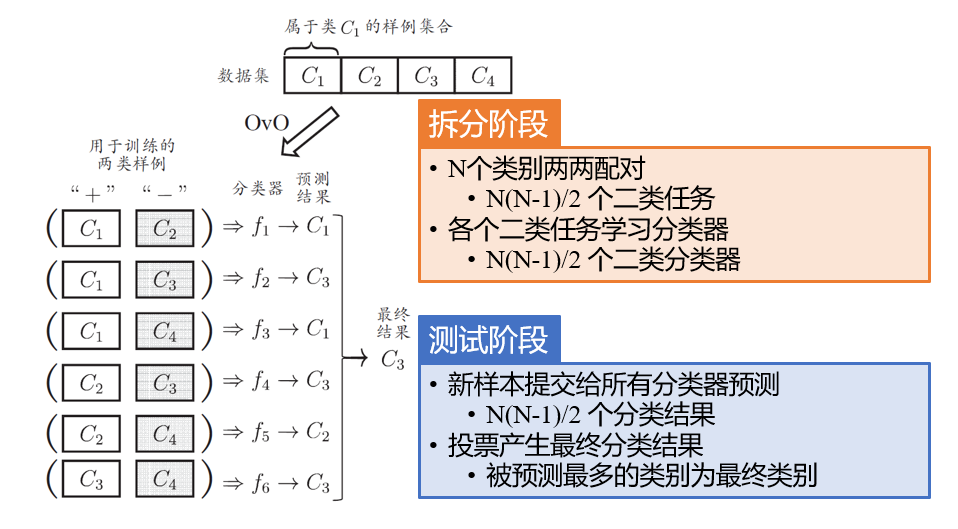
\includegraphics[scale=0.5]{1.png}
\end{figure}

\begin{figure}[H]
    \centering
    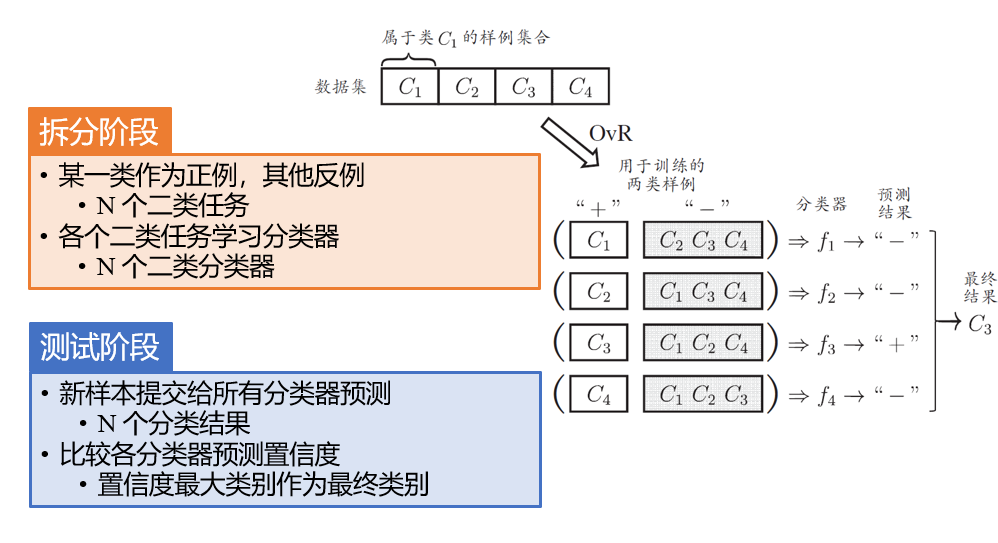
\includegraphics[scale=0.5]{2.png}
\end{figure}
\subsubsection{神经网络}
本次实验中只使用了含有一个隐藏层的MLP模型,MLP又称多层感知机,除了输入输出层以外,它中间可以含有多个隐藏层,
最简单的MLP模型只有一个隐藏层。

多层感知机的层与层是全连接的,每个神经元都接受若干个输入并计算得到若干个输出传向下一层的神经元。通常我们通过
误差逆传播(BP)算法来求解感知机中各项参数。
\begin{figure}[H]
    \centering
    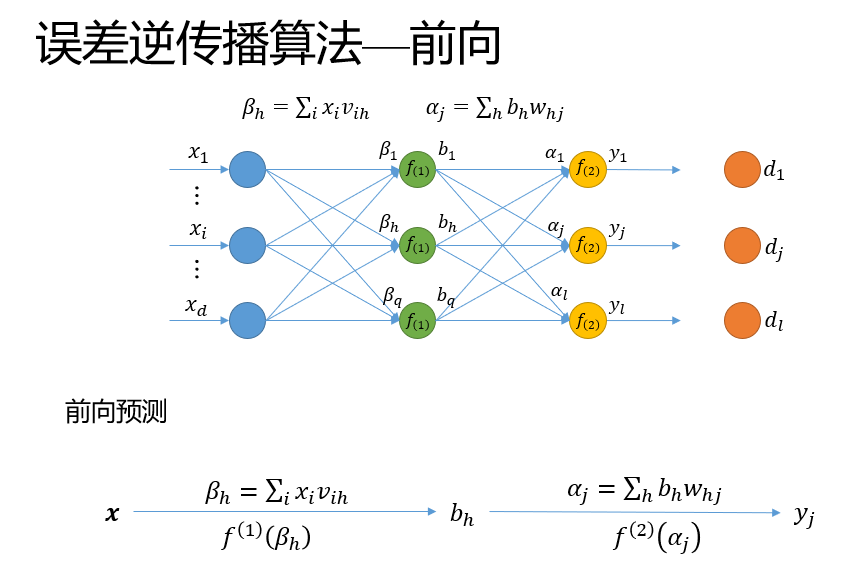
\includegraphics[scale=0.4]{3.png}
\end{figure}
\begin{figure}[H]
    \centering
    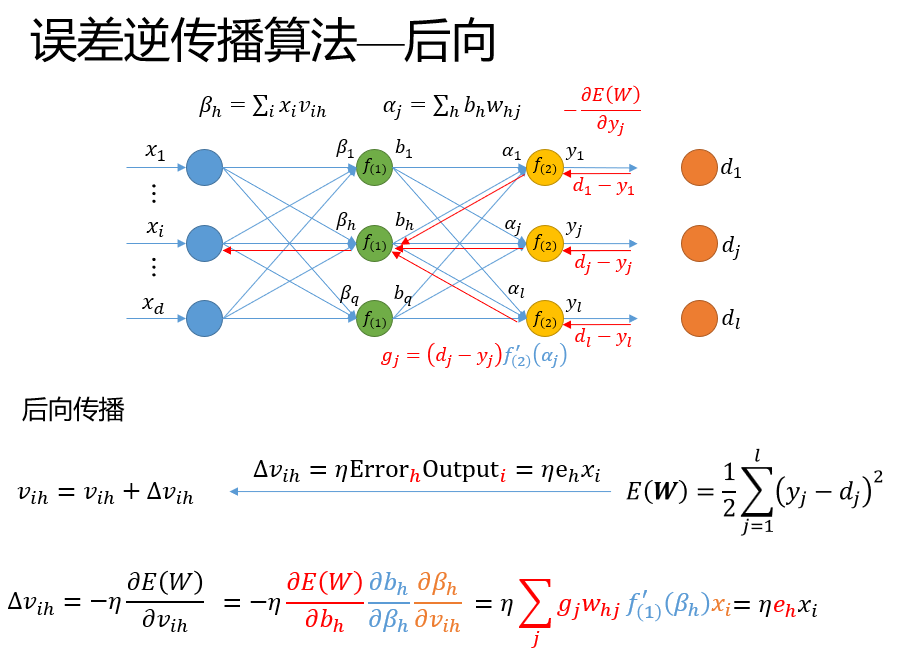
\includegraphics[scale=0.4]{4.png}
\end{figure}
\subsubsection{决策树与XGBoost}
详见\href{https://github.com/xiaoma-ustc/2022-USTC-Introduction-to-Machine-Learning/blob/main/lab/lab3/report/report.pdf}{决策树与XGBoost}
\subsubsection{支持向量机}
详见\href{https://github.com/xiaoma-ustc/2022-USTC-Introduction-to-Machine-Learning/blob/main/lab/lab2/report/Report.pdf}{支持向量机}
\section{实验步骤}
\subsection{数据预处理}
\begin{itemize}
    \item 首先对查看数据集的信息,发现其存在缺失值,考虑到样本数量充足且有缺失值的样本量较少,故使用\textbf{pandas.dropna函数}将具有缺失值的样本舍弃。
    \item 对数据进行归一化,考虑到数据可能存在噪声,使用\textbf{sklearn.covariance.EllipticEnvelope函数}进行噪声检测,并将检测到的噪声样本舍弃。
    \item 考虑到使用整个数据集训练模型计算量过大且可能存在与分类任务相关性较低的特征,故对数据进行特征提取,分别使用\textbf{shap库}和\textbf{XGboost.plot\_importance函数}选择权重最大的特征进行切片。
\end{itemize}
\subsection{模型训练}
首次训练未进行特征提取,所有模型的精确度都在0.25左右。

然后使用过滤法进行特征提取,分别使用卡方分布,F分布,Pearson相关系数等过滤特征,
发现在卡方分布下,神经网络模型的精确度为0.267,其他模型的精度仍在0.25左右。

\begin{lstlisting}
    neu_net_classfier = MLPClassifier(hidden_layer_sizes=(20,),
                                max_iter = 1000,
                                activation='relu',
                                solver = 'adam',
                                alpha = 0.0001,
                                )
\end{lstlisting}

接下来进行嵌入法进行特征提取,使用基于XGBoost模型的特征提取,模型参数如下
\begin{lstlisting}
    model = XGBClassifier(learning_rate = 1,
                            booster = 'gbtree',
                            max_depth = 20,
                            num_class = 4,
                            gamma = 0.1,
                            subsample = 1,
                            objective = 'muti:softprob',
                            eval_metric = 'mlogloss',
                            use_label_encoder = False,)
\end{lstlisting}
使用\textbf{shap.summary\_plot(shap\_values, data, plot\_type="bar")}得到的条形图如下所示
\begin{figure}[H]
    \centering
    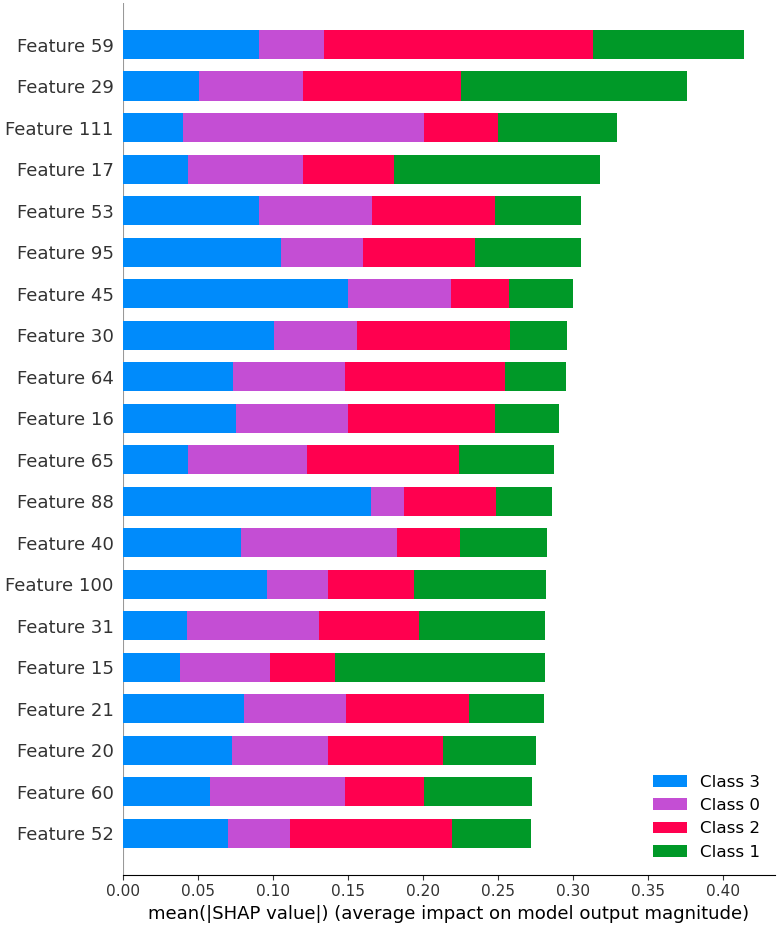
\includegraphics[scale=0.6]{5.png}
\end{figure}
使用\textbf{plot\_importance(importance\_type='gain')}得到的条形图如下所示
\begin{figure}[H]
    \centering
    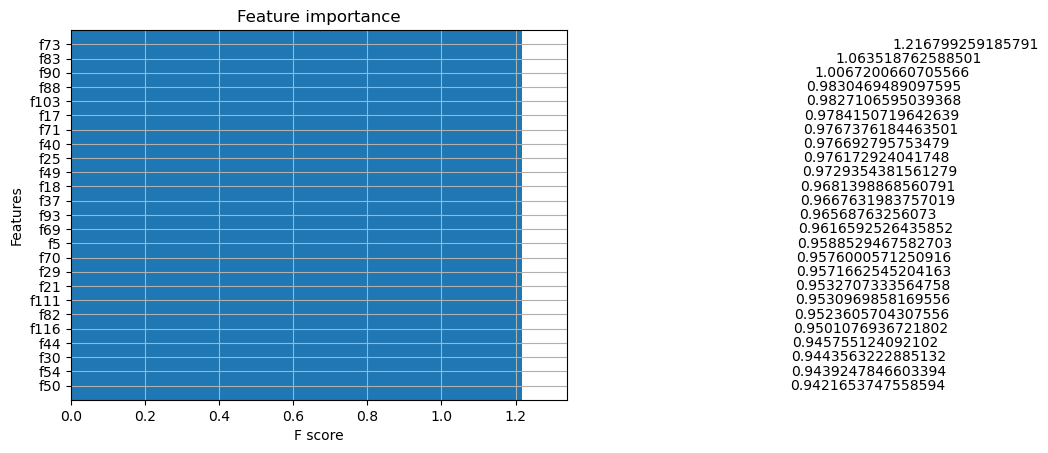
\includegraphics[scale=0.6]{6.png}
\end{figure}
分别选择两图中权重较高的特征进行训练,得到的所有模型的精度仍在0.25左右。

继续进行特征提取,更改参数
\begin{lstlisting}
    model = XGBClassifier(learning_rate = 0.1,
                            booster = 'gbtree',
                            max_depth = 20,
                            num_class = 4,
                            gamma = 0.1,
                            subsample = 1,
                            objective = 'muti:softprob',
                            eval_metric = 'mlogloss',
                            use_label_encoder = False,)
\end{lstlisting}
使用\textbf{shap.summary\_plot(shap\_values, data, plot\_type="bar")}得到的条形图如下所示
\begin{figure}[H]
    \centering
    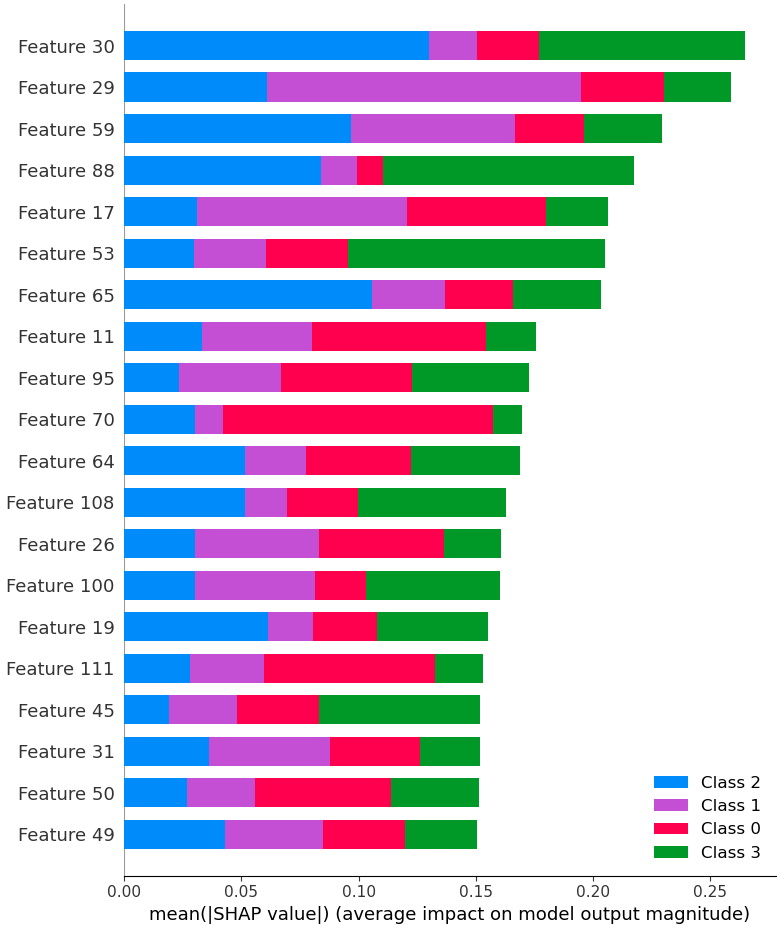
\includegraphics[scale=0.6]{7.png}
\end{figure}
使用\textbf{plot\_importance(importance\_type='gain')}得到的条形图如下所示
\begin{figure}[H]
    \centering
    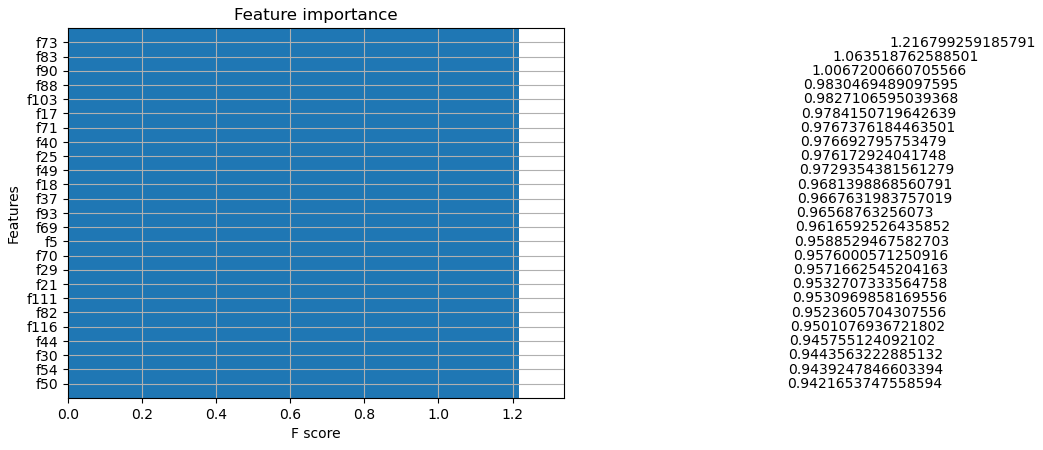
\includegraphics[scale=0.6]{8.png}
\end{figure}
分别选择两图中权重较高的特征进行训练,发现当选择特征为[73, 90, 83, 88, 103, 17, 71, 40, 25]时,XGBoost模型的精确度达到0.26,其他模型的精确度仍为0.25左右。

按照该方式不断调整,最终发现在该参数下
\begin{lstlisting}
    model = XGBClassifier(learning_rate = 0.1,
                            booster = 'gbtree',
                            max_depth = 20,
                            num_class = 4,
                            gamma = 2,
                            subsample = 1,
                            objective = 'muti:softprob',
                            eval_metric = 'mlogloss',
                            use_label_encoder = False,)
\end{lstlisting}
使用\textbf{shap.summary\_plot(shap\_values, data, plot\_type="bar")}得到的条形图如下所示
\begin{figure}[H]
    \centering
    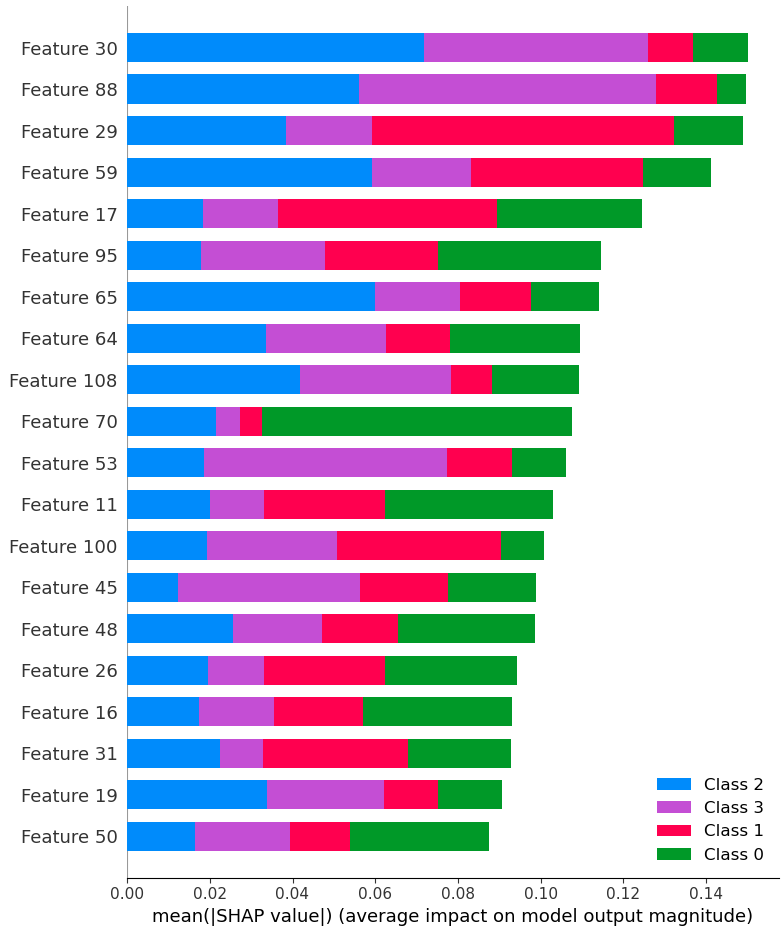
\includegraphics[scale=0.6]{9.png}
\end{figure}
使用\textbf{plot\_importance(importance\_type='gain')}得到的条形图如下所示
\begin{figure}[H]
    \centering
    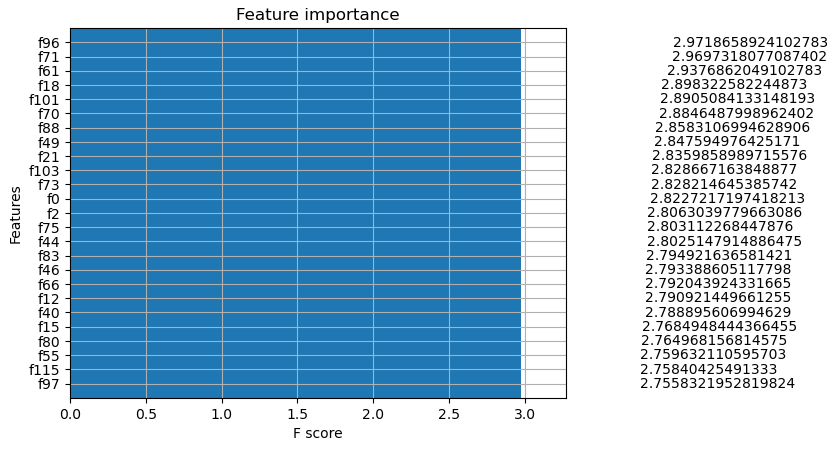
\includegraphics[scale=0.6]{10.png}
\end{figure}
发现当选择特征为30, 29, 59, 88, 17, 53, 65时,XGBoost模型的精确度达到0.268,其他模型的精确度仍为0.25左右。
\section{实验分析}

实验所提供的数据集存在大量的无价值特征,可以通过特征选择的方法来提取有价值的特征进行模型训练以达到更好的结果,由于本人能力有限,无法提取出使模型表现非常好的特征组合。
\end{document}